\section{模板简介}

本模板基于$\LaTeXe$。$\LaTeXe$目前来说主流的地位不可撼动,已有的解决方案多。

$\LaTeXe$编译引擎用xeLaTeX,基于“内容和格式相分离”的理念,格式和内容分开。

将源文件分割成若干个文件,例如将每章内容单独写在一个文件中,会大大简化修改和校对的工作。重新编译最好删除辅助文件,特别是遇到目录、参考文献有报错的时候。双击del.bat文件即可删除辅助文件。




\subsection{封面}

需要在main.tex文件的导言区修改以下个人信息,然后在正文部分使用\verb|\Cover|制作封面。

\begin{lstlisting}
	%封面、中文摘要信息
	\myname{你的名字}
	\studentid{你的学号}
	\major{你的专业}
	\thesis{你的论文题目}
	\department{理学院}
	\mysupervisor{你的导师}
	\class{所在班级}
\end{lstlisting}


\subsection{诚信承诺书和任务书}

将你的诚信承诺书转成pdf文件后放入pdf文件夹

\begin{lstlisting}
	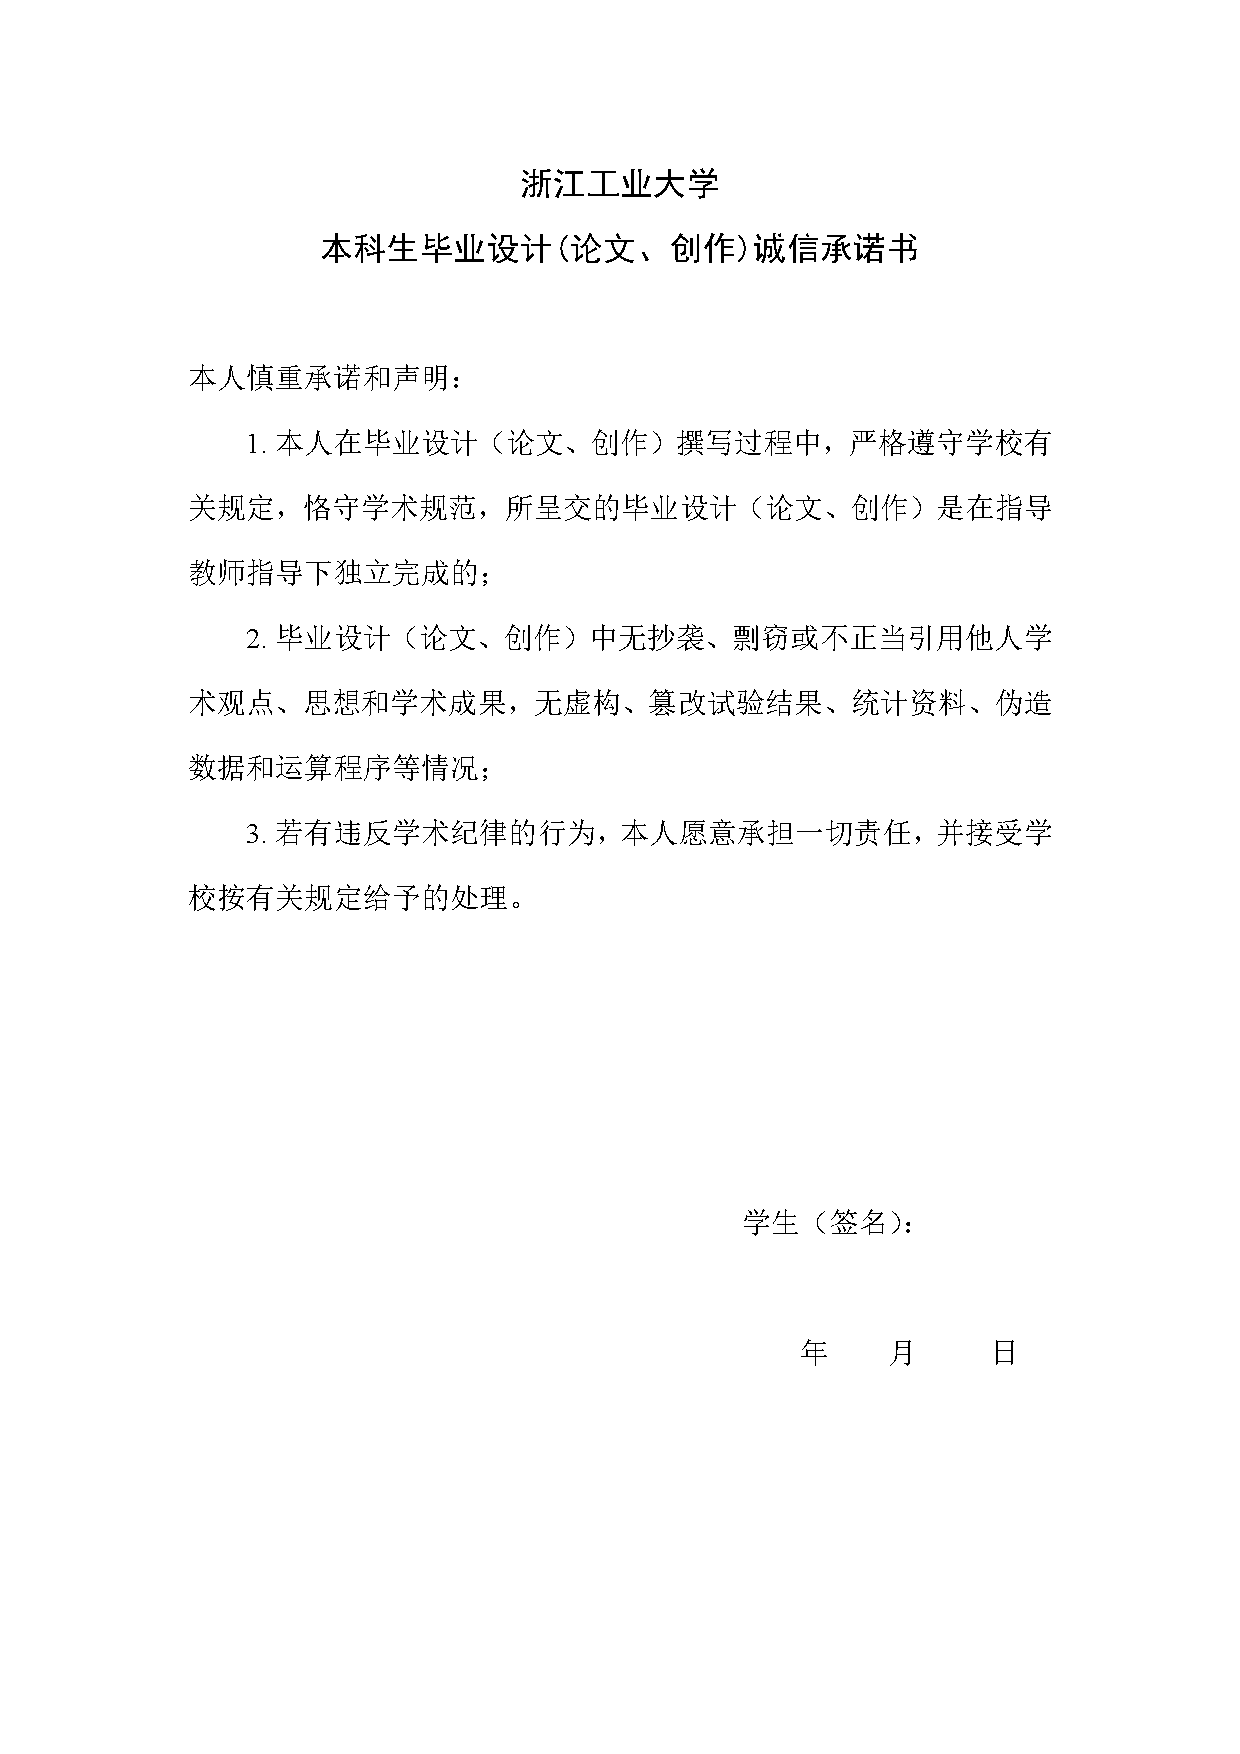
\includepdf{pdf/诚信承诺书.pdf}
	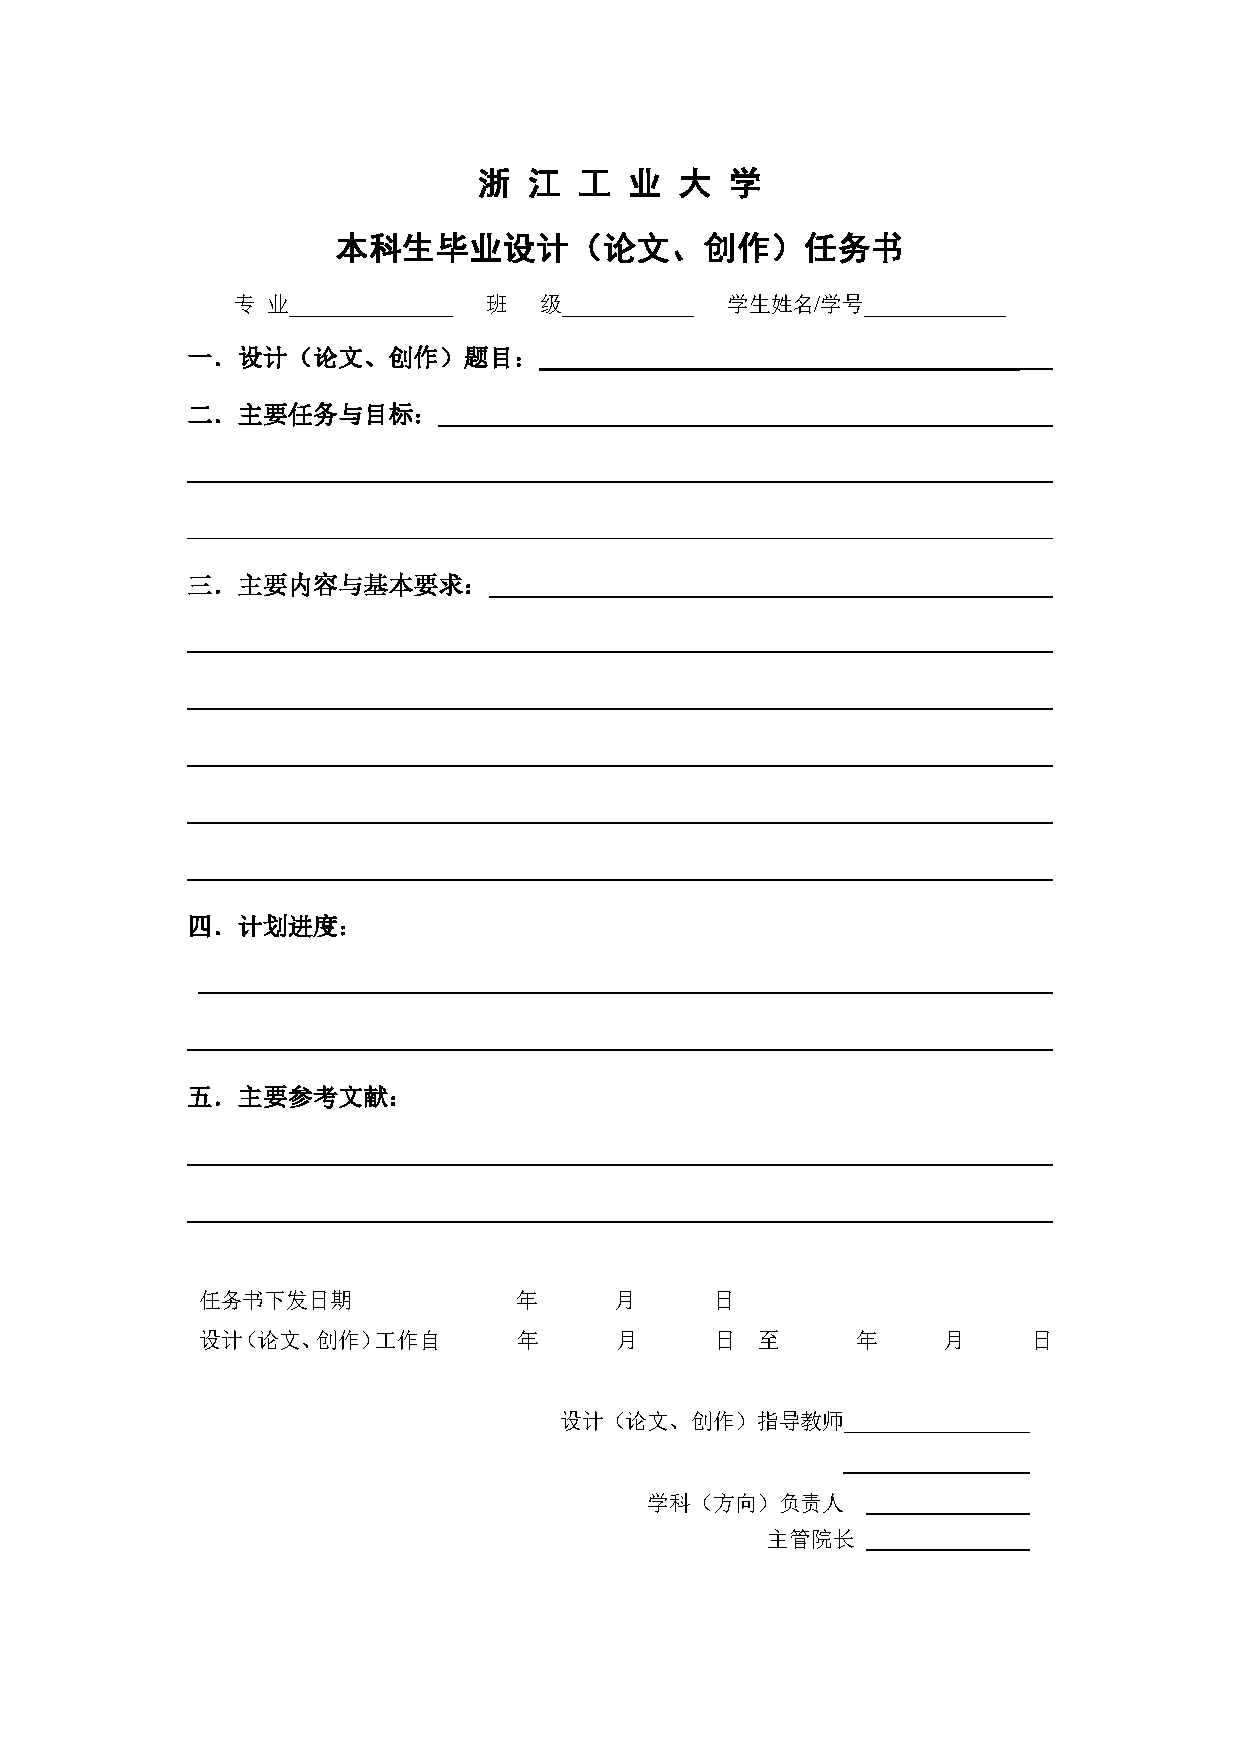
\includepdf{pdf/任务书.pdf}
\end{lstlisting}

\subsection{摘要}

需要在main.tex文件的导言区修改以下个人信息:

\begin{lstlisting}
	%英文摘要信息
	\Enthesis{你的英文摘要标题}
	\Enmyname{你的英文名}
	\Enmysupervisor{导师的英文名}
	\Endepartment{College of Science}
\end{lstlisting}

在\verb|\ZhAbstract{中文摘要内容}{关键词1\hspace{1em}关键词2}|中第一个花括号中写入中文摘要,在第二个花括号中填入关键词

在\verb|\EnAbstract{Contents of English Abstract}{Keywords1;Keywords2;}|中第一个花括号中写入英文摘要,在第二个花括号中填入英文关键词


\subsection{目录、图列、表列}

以下是目录、表列、图列的生成,以及之后的页码用阿拉伯数字,不需要更改。不需要人为添加,插入图片、表格时会自动生成索引。

\begin{lstlisting}
	%目录,表列、图列
	\makeTOCandLOTandLOF
	%页码计数器清零,阿拉伯数字
	\setcounter{page}{0}
	\pagenumbering{arabic}
	\newpage
\end{lstlisting}

\subsection{正文}

将源文件分割成若干个文件,例如将每章内容单独写在一个文件中,会大大简化修改和校对的工作。建议把每个章节放在parts文件夹中,用\verb|\input{parts/xxxx}|来导入,不需要加.tex后缀。

\begin{lstlisting}
	\section{绪论}


\subsection{研究动机与目的}

\subsection{研究背景}


\subsection{研究方法}

\subsection{论文内容概述}

\subsubsection{三级标题}

\paragraph{\noindent 四级标题}

\newpage


	\section{模板简介}

本模板基于$\LaTeXe$。$\LaTeXe$目前来说主流的地位不可撼动,已有的解决方案多。

$\LaTeXe$编译引擎用xeLaTeX,基于“内容和格式相分离”的理念,格式和内容分开。

将源文件分割成若干个文件,例如将每章内容单独写在一个文件中,会大大简化修改和校对的工作。重新编译最好删除辅助文件,特别是遇到目录、参考文献有报错的时候。双击del.bat文件即可删除辅助文件。




\subsection{封面}

需要在main.tex文件的导言区修改以下个人信息,然后在正文部分使用\verb|\Cover|制作封面。

\begin{lstlisting}
	%封面、中文摘要信息
	\myname{你的名字}
	\studentid{你的学号}
	\major{你的专业}
	\thesis{你的论文题目}
	\department{理学院}
	\mysupervisor{你的导师}
	\class{所在班级}
\end{lstlisting}


\subsection{诚信承诺书}

将你的诚信承诺书转成pdf文件后放入pdf文件夹

\begin{lstlisting}
	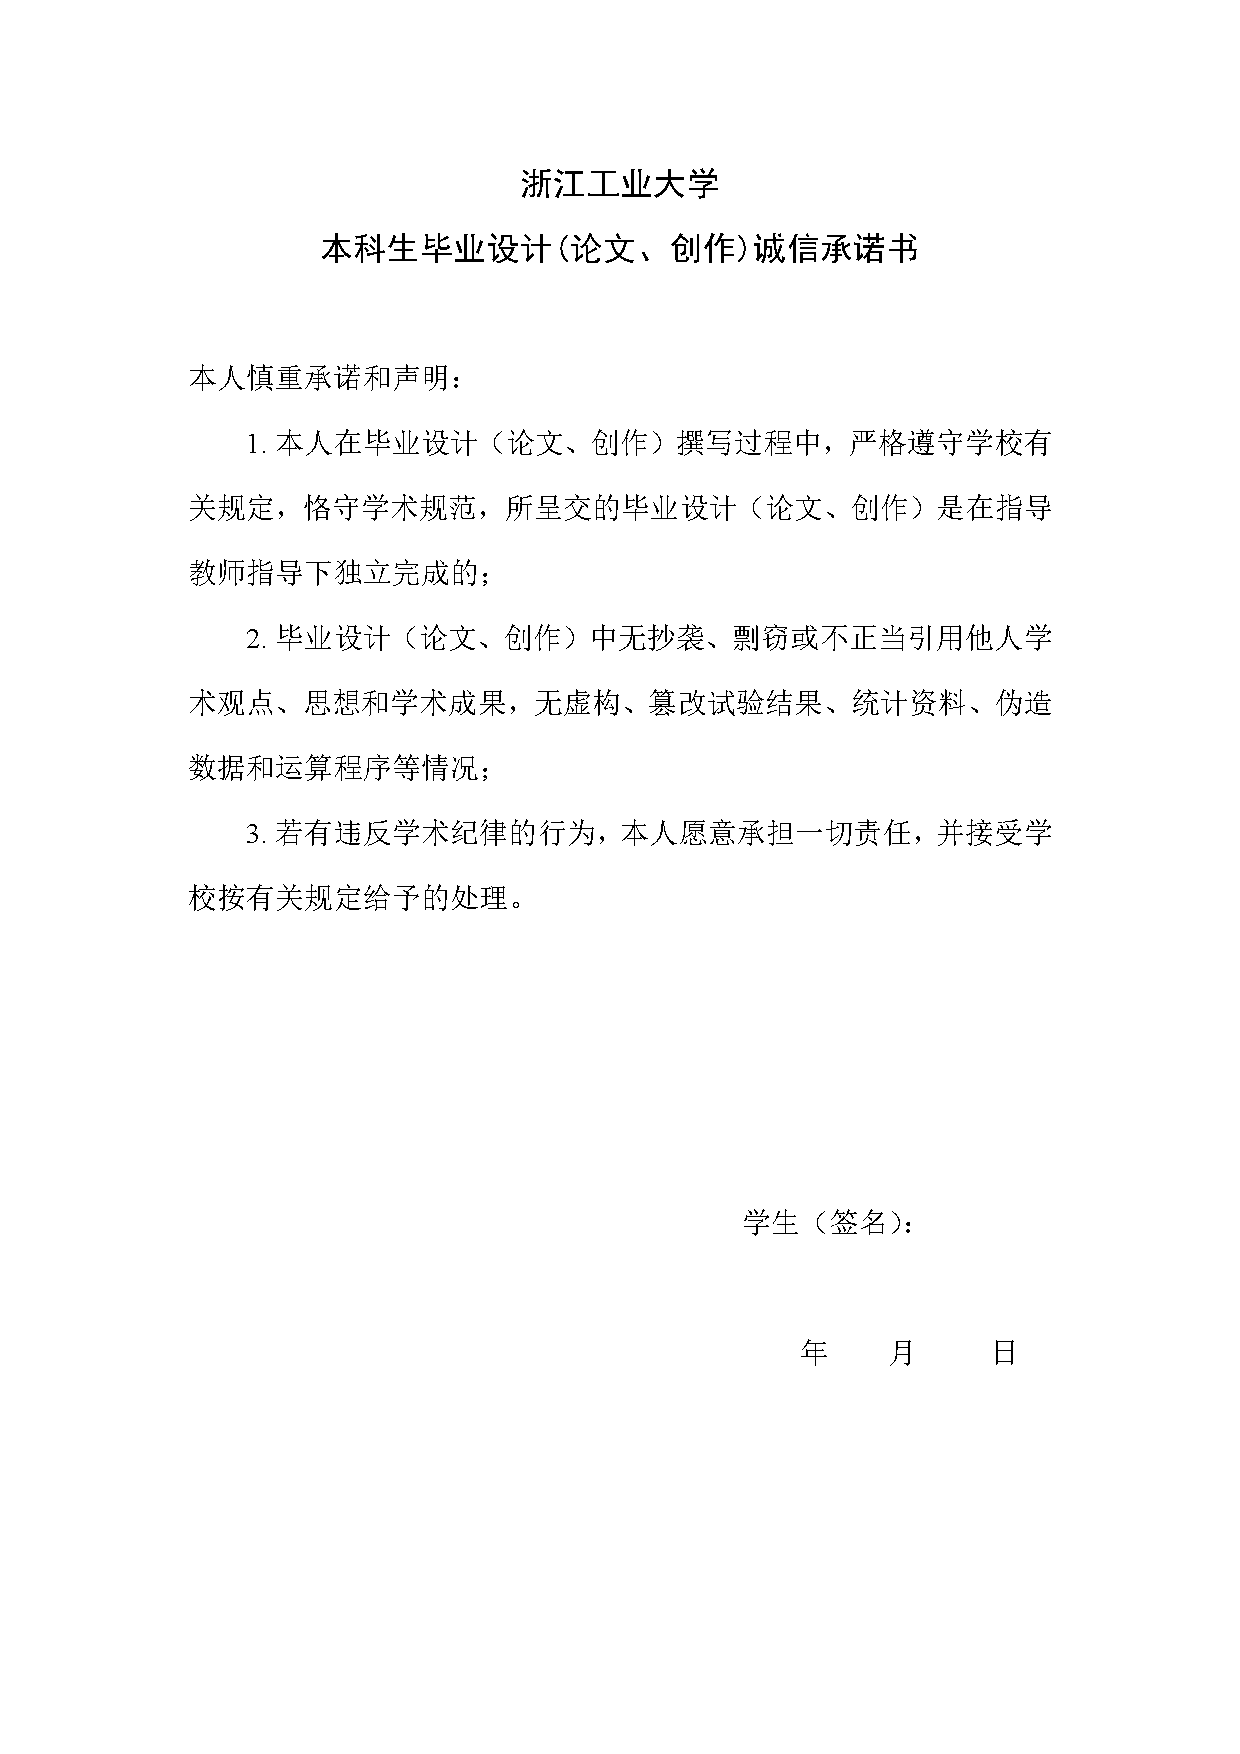
\includepdf{pdf/诚信承诺书.pdf}
	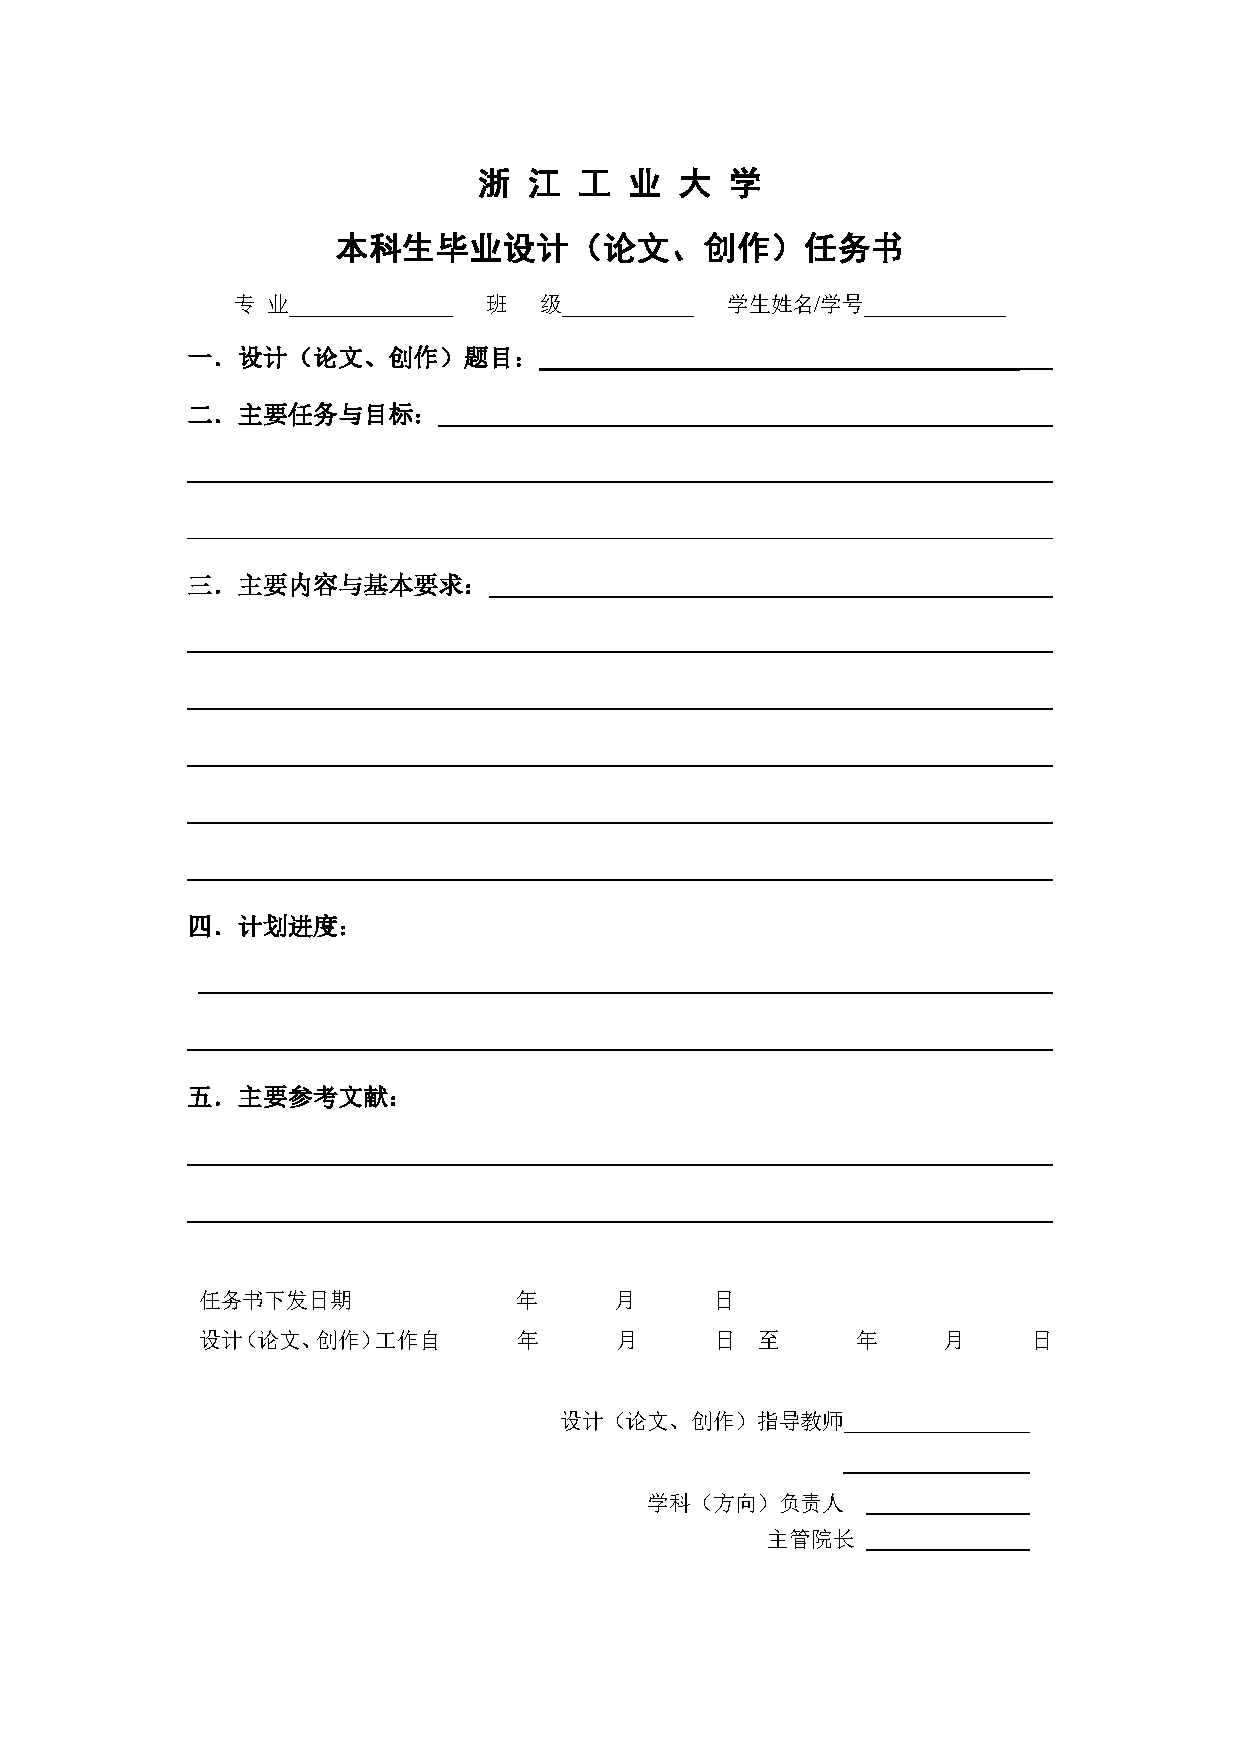
\includepdf{pdf/任务书.pdf}
\end{lstlisting}

\subsection{摘要}

需要在main.tex文件的导言区修改以下个人信息:

\begin{lstlisting}
	%英文摘要信息
	\Enthesis{你的英文摘要标题}
	\Enmyname{你的英文名}
	\Enmysupervisor{导师的英文名}
	\Endepartment{College of Science}
\end{lstlisting}

在\verb|\ZhAbstract{中文摘要内容}{关键词1\hspace{1em}关键词2|中第一个花括号中写入中文摘要,在第二个花括号中填入关键词

在\verb|\EnAbstract{Contents of English Abstract}{Keywords1;Keywords2;}|中第一个花括号中写入英文摘要,在第二个花括号中填入英文关键词


\subsection{目录、图列、表列}

以下是目录、表列、图列的生成,以及之后的页码用阿拉伯数字,不需要更改。不需要人为添加,插入图片、表格时会自动生成索引。

\begin{lstlisting}
	%目录,表列、图列
	\makeTOCandLOTandLOF
	%页码计数器清零,阿拉伯数字
	\setcounter{page}{0}
	\pagenumbering{arabic}
	\newpage
\end{lstlisting}

\subsection{正文}

将源文件分割成若干个文件,例如将每章内容单独写在一个文件中,会大大简化修改和校对的工作。建议把每个章节放在parts文件夹中,用\verb|\input{parts/xxxx}|来导入,不需要加.tex后缀。

\begin{lstlisting}
	\section{绪论}


\subsection{研究动机与目的}

\subsection{研究背景}


\subsection{研究方法}

\subsection{论文内容概述}

\subsubsection{三级标题}

\paragraph{\noindent 四级标题}

\newpage


	\section{模板简介}

本模板基于$\LaTeXe$。$\LaTeXe$目前来说主流的地位不可撼动,已有的解决方案多。

$\LaTeXe$编译引擎用xeLaTeX,基于“内容和格式相分离”的理念,格式和内容分开。

将源文件分割成若干个文件,例如将每章内容单独写在一个文件中,会大大简化修改和校对的工作。重新编译最好删除辅助文件,特别是遇到目录、参考文献有报错的时候。双击del.bat文件即可删除辅助文件。




\subsection{封面}

需要在main.tex文件的导言区修改以下个人信息,然后在正文部分使用\verb|\Cover|制作封面。

\begin{lstlisting}
	%封面、中文摘要信息
	\myname{你的名字}
	\studentid{你的学号}
	\major{你的专业}
	\thesis{你的论文题目}
	\department{理学院}
	\mysupervisor{你的导师}
	\class{所在班级}
\end{lstlisting}


\subsection{诚信承诺书}

将你的诚信承诺书转成pdf文件后放入pdf文件夹

\begin{lstlisting}
	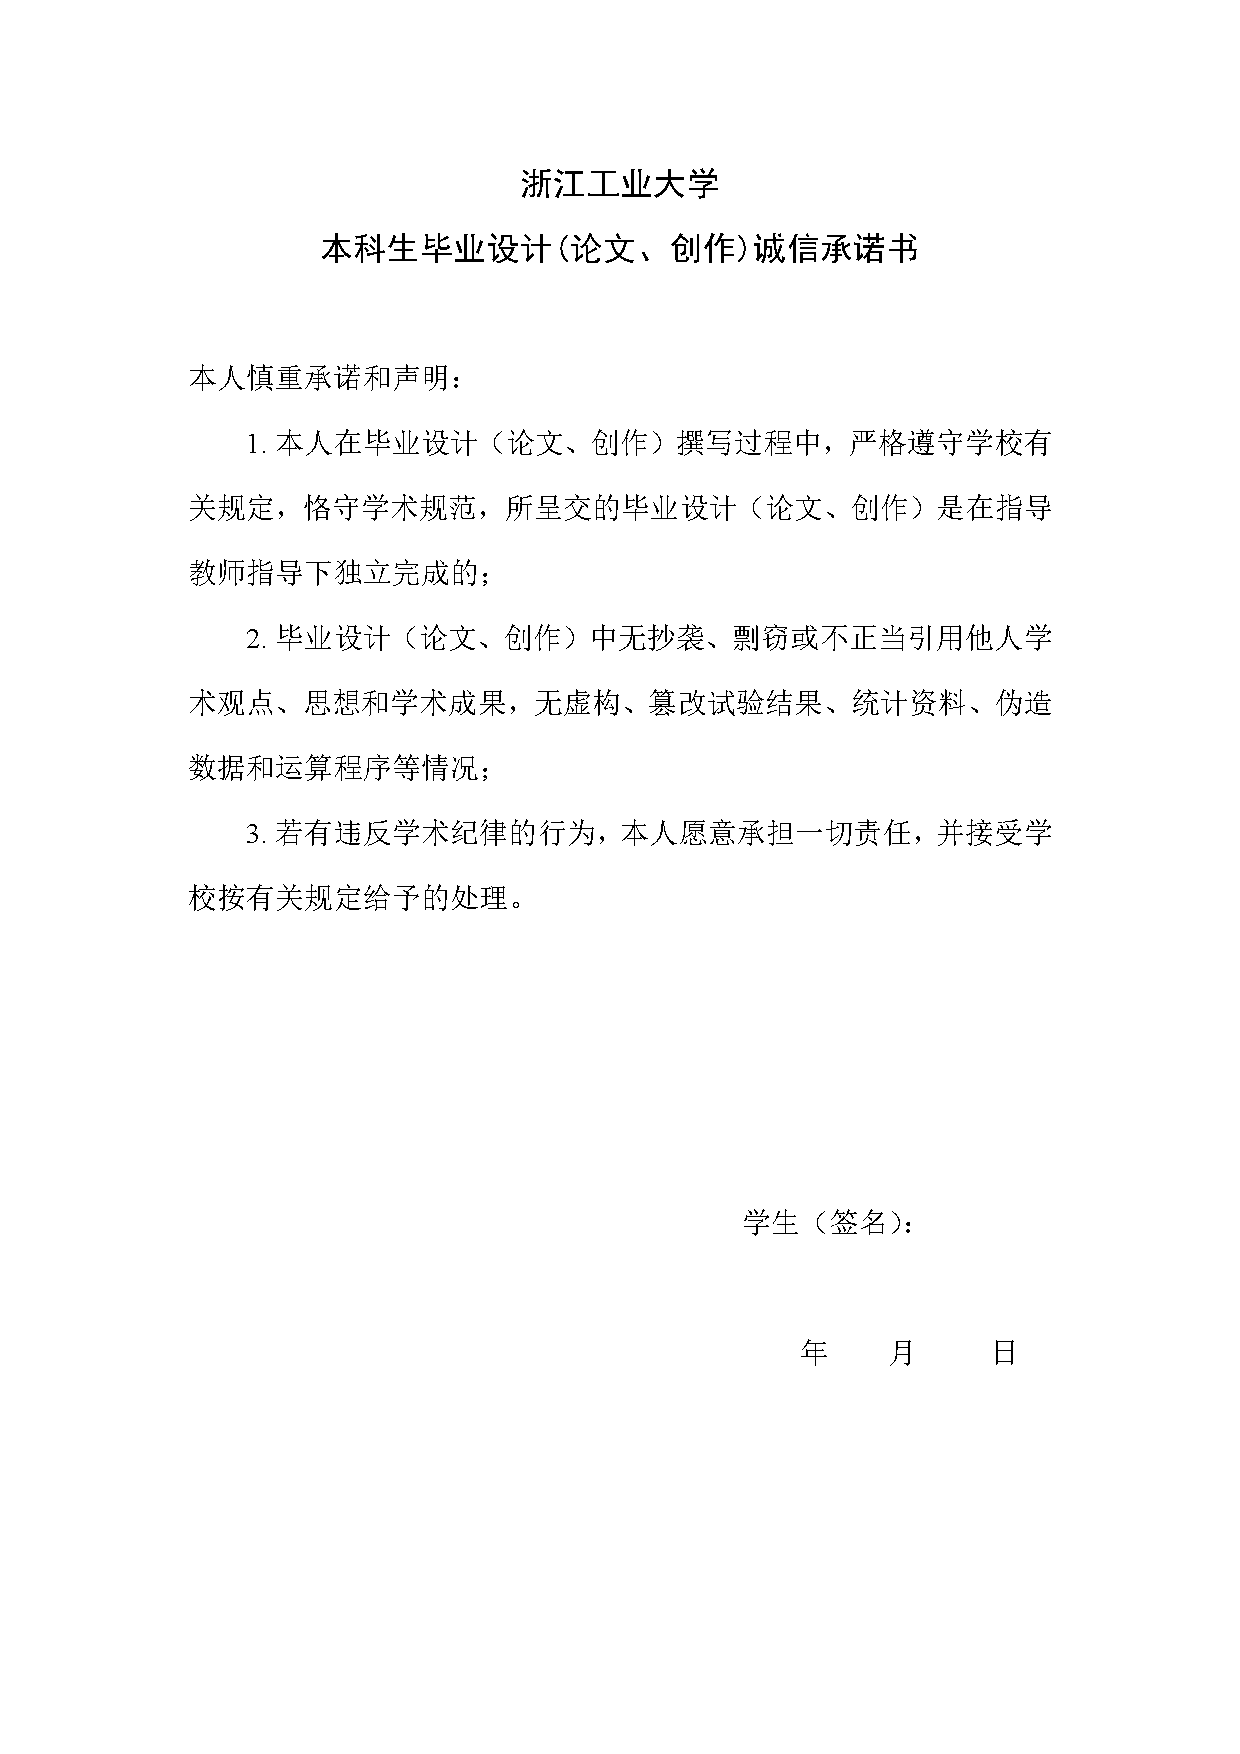
\includepdf{pdf/诚信承诺书.pdf}
	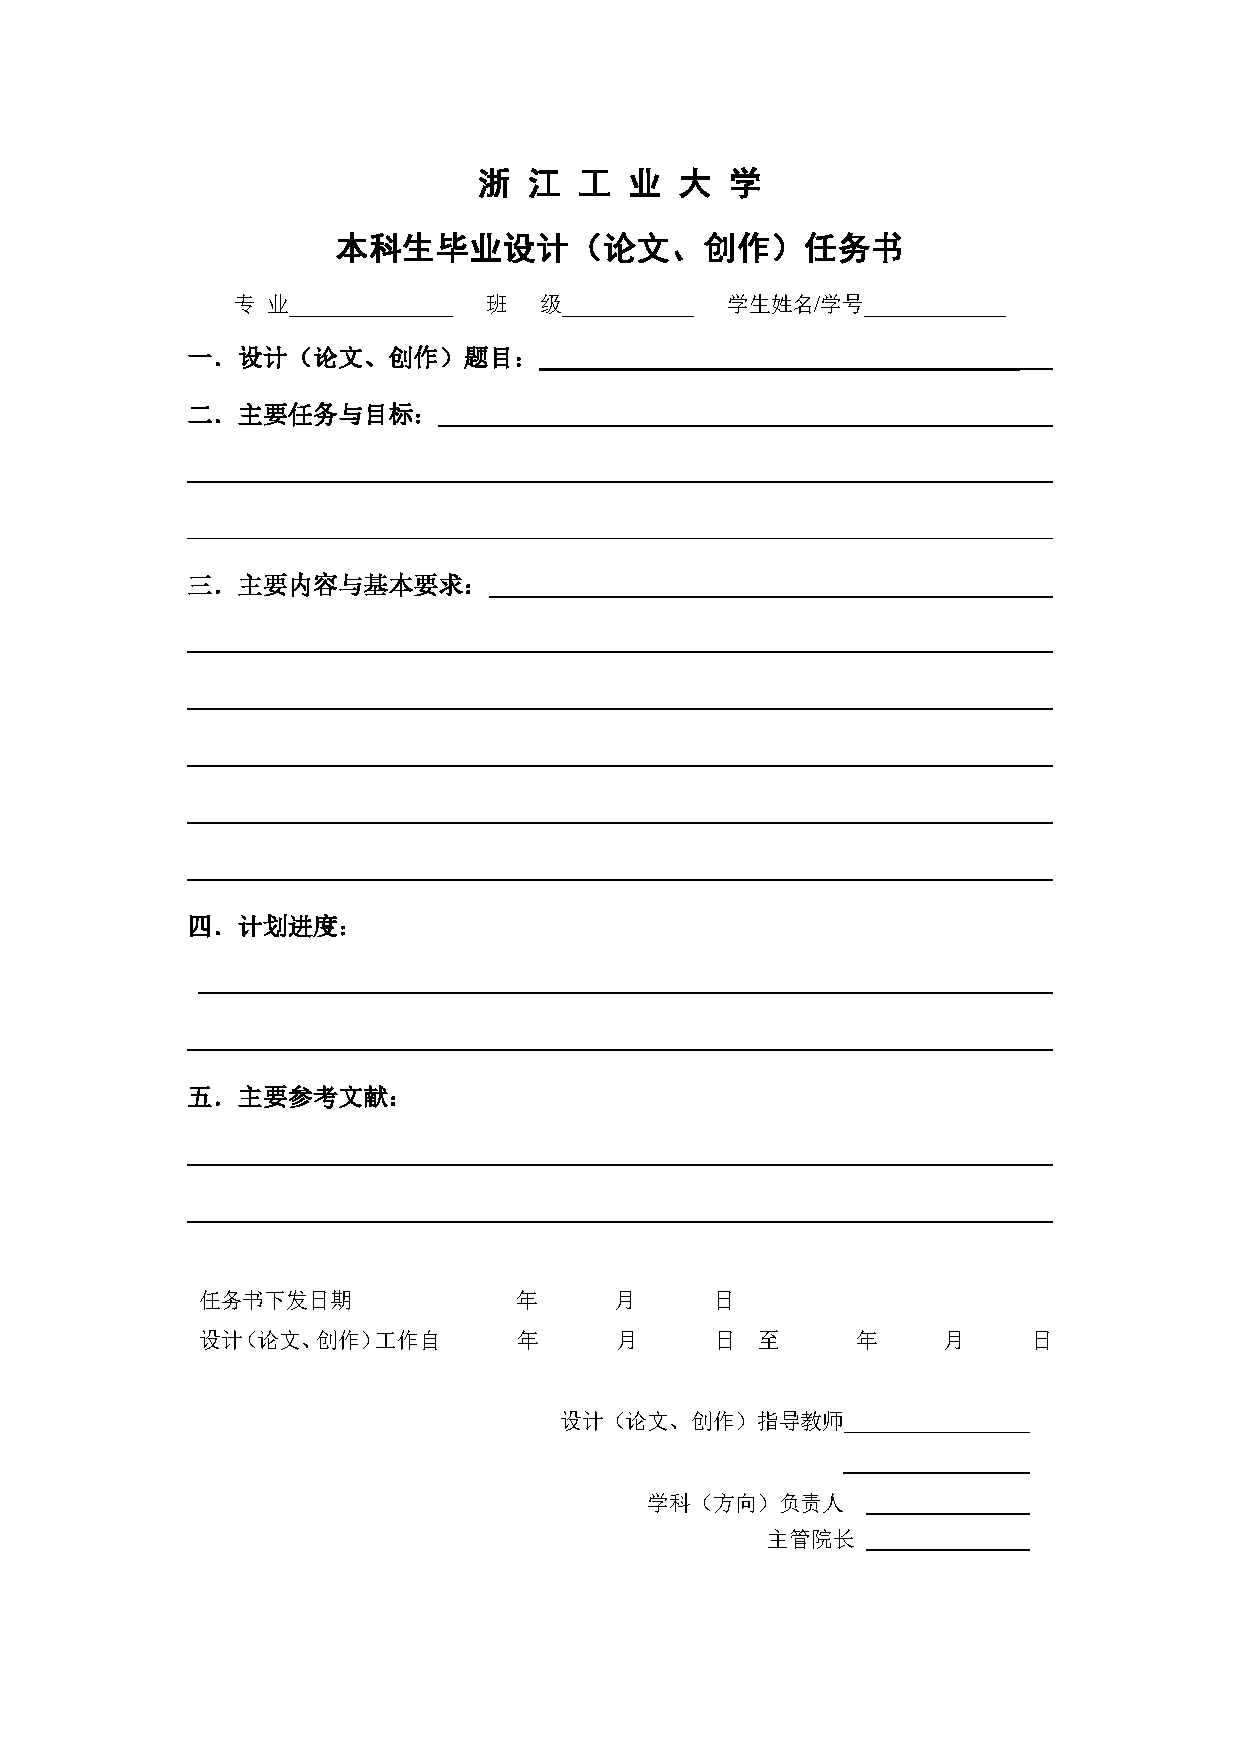
\includepdf{pdf/任务书.pdf}
\end{lstlisting}

\subsection{摘要}

需要在main.tex文件的导言区修改以下个人信息:

\begin{lstlisting}
	%英文摘要信息
	\Enthesis{你的英文摘要标题}
	\Enmyname{你的英文名}
	\Enmysupervisor{导师的英文名}
	\Endepartment{College of Science}
\end{lstlisting}

在\verb|\ZhAbstract{中文摘要内容}{关键词1\hspace{1em}关键词2|中第一个花括号中写入中文摘要,在第二个花括号中填入关键词

在\verb|\EnAbstract{Contents of English Abstract}{Keywords1;Keywords2;}|中第一个花括号中写入英文摘要,在第二个花括号中填入英文关键词


\subsection{目录、图列、表列}

以下是目录、表列、图列的生成,以及之后的页码用阿拉伯数字,不需要更改。不需要人为添加,插入图片、表格时会自动生成索引。

\begin{lstlisting}
	%目录,表列、图列
	\makeTOCandLOTandLOF
	%页码计数器清零,阿拉伯数字
	\setcounter{page}{0}
	\pagenumbering{arabic}
	\newpage
\end{lstlisting}

\subsection{正文}

将源文件分割成若干个文件,例如将每章内容单独写在一个文件中,会大大简化修改和校对的工作。建议把每个章节放在parts文件夹中,用\verb|\input{parts/xxxx}|来导入,不需要加.tex后缀。

\begin{lstlisting}
	\section{绪论}


\subsection{研究动机与目的}

\subsection{研究背景}


\subsection{研究方法}

\subsection{论文内容概述}

\subsubsection{三级标题}

\paragraph{\noindent 四级标题}

\newpage


	\section{模板简介}

本模板基于$\LaTeXe$。$\LaTeXe$目前来说主流的地位不可撼动,已有的解决方案多。

$\LaTeXe$编译引擎用xeLaTeX,基于“内容和格式相分离”的理念,格式和内容分开。

将源文件分割成若干个文件,例如将每章内容单独写在一个文件中,会大大简化修改和校对的工作。重新编译最好删除辅助文件,特别是遇到目录、参考文献有报错的时候。双击del.bat文件即可删除辅助文件。




\subsection{封面}

需要在main.tex文件的导言区修改以下个人信息,然后在正文部分使用\verb|\Cover|制作封面。

\begin{lstlisting}
	%封面、中文摘要信息
	\myname{你的名字}
	\studentid{你的学号}
	\major{你的专业}
	\thesis{你的论文题目}
	\department{理学院}
	\mysupervisor{你的导师}
	\class{所在班级}
\end{lstlisting}


\subsection{诚信承诺书}

将你的诚信承诺书转成pdf文件后放入pdf文件夹

\begin{lstlisting}
	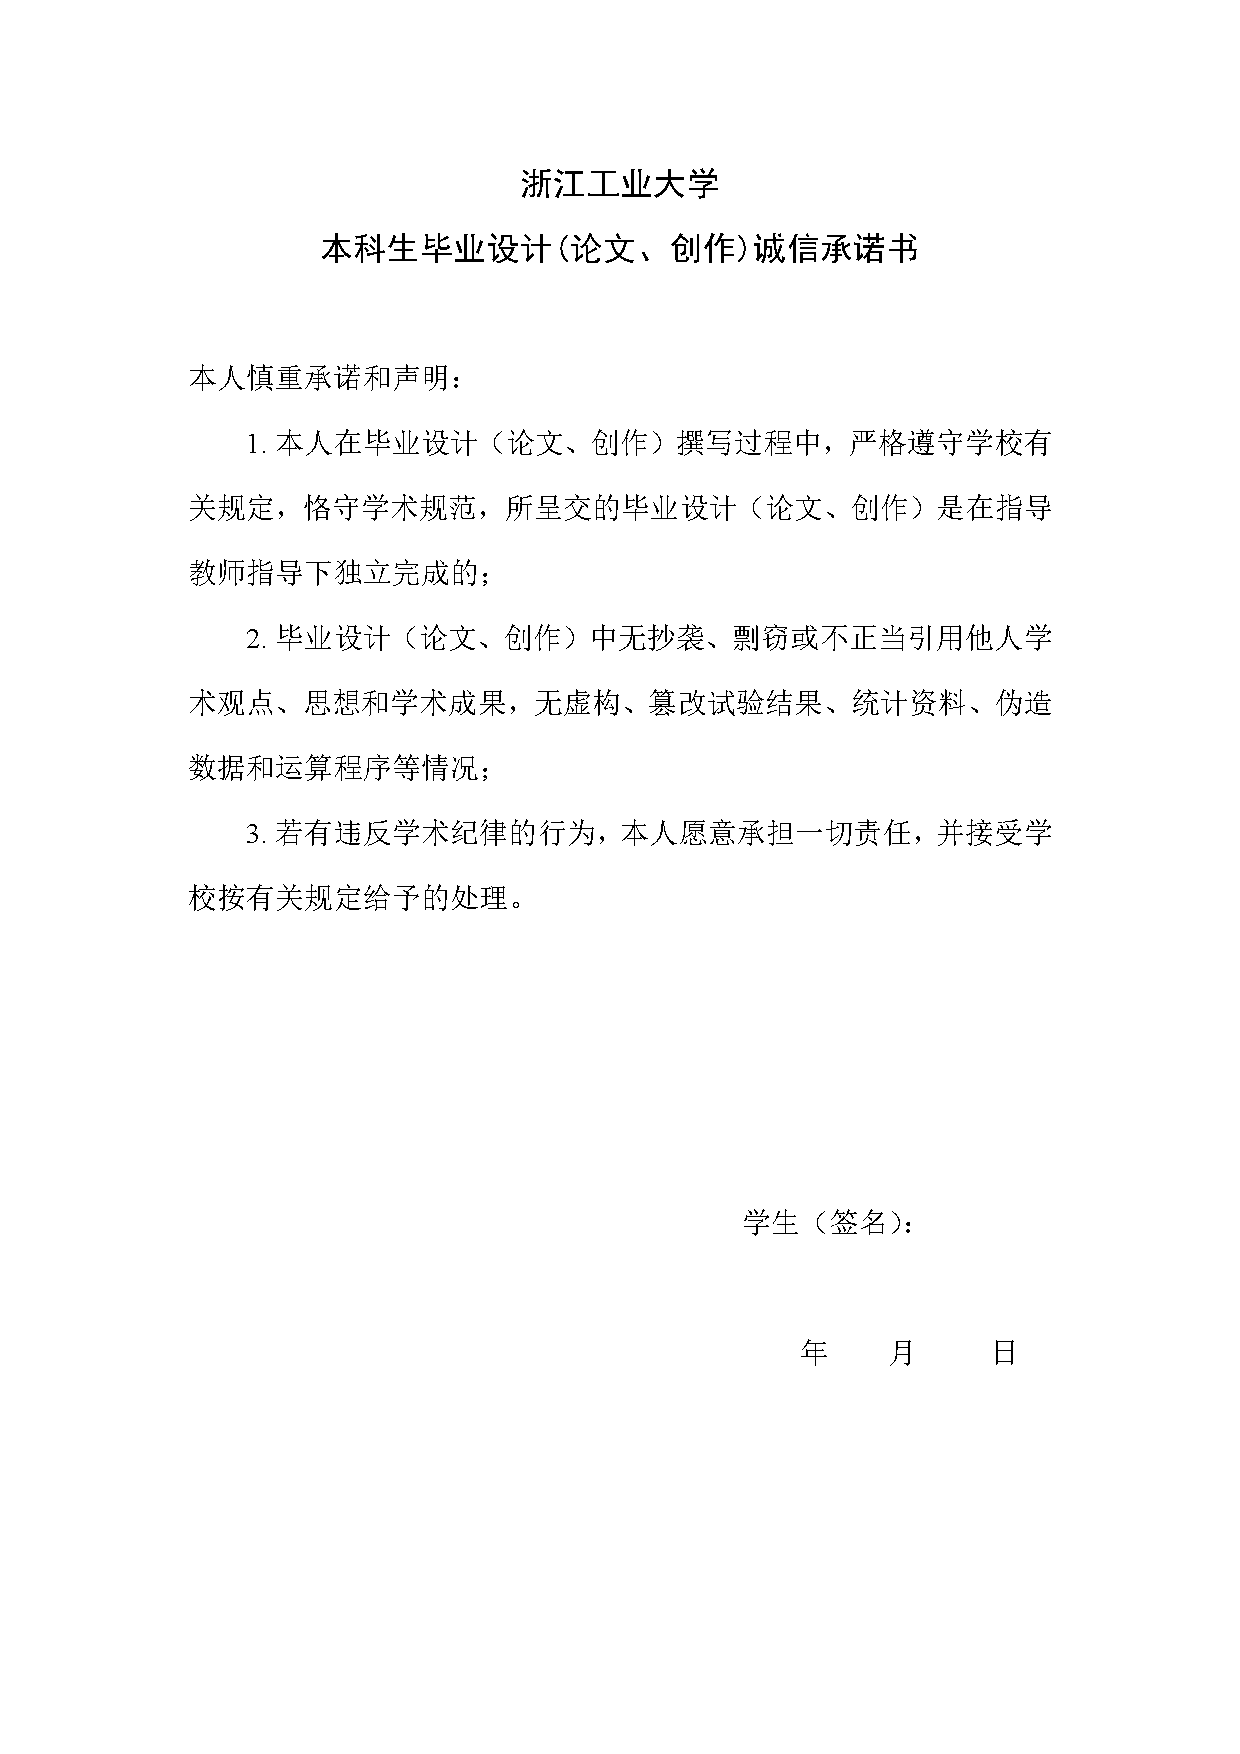
\includepdf{pdf/诚信承诺书.pdf}
	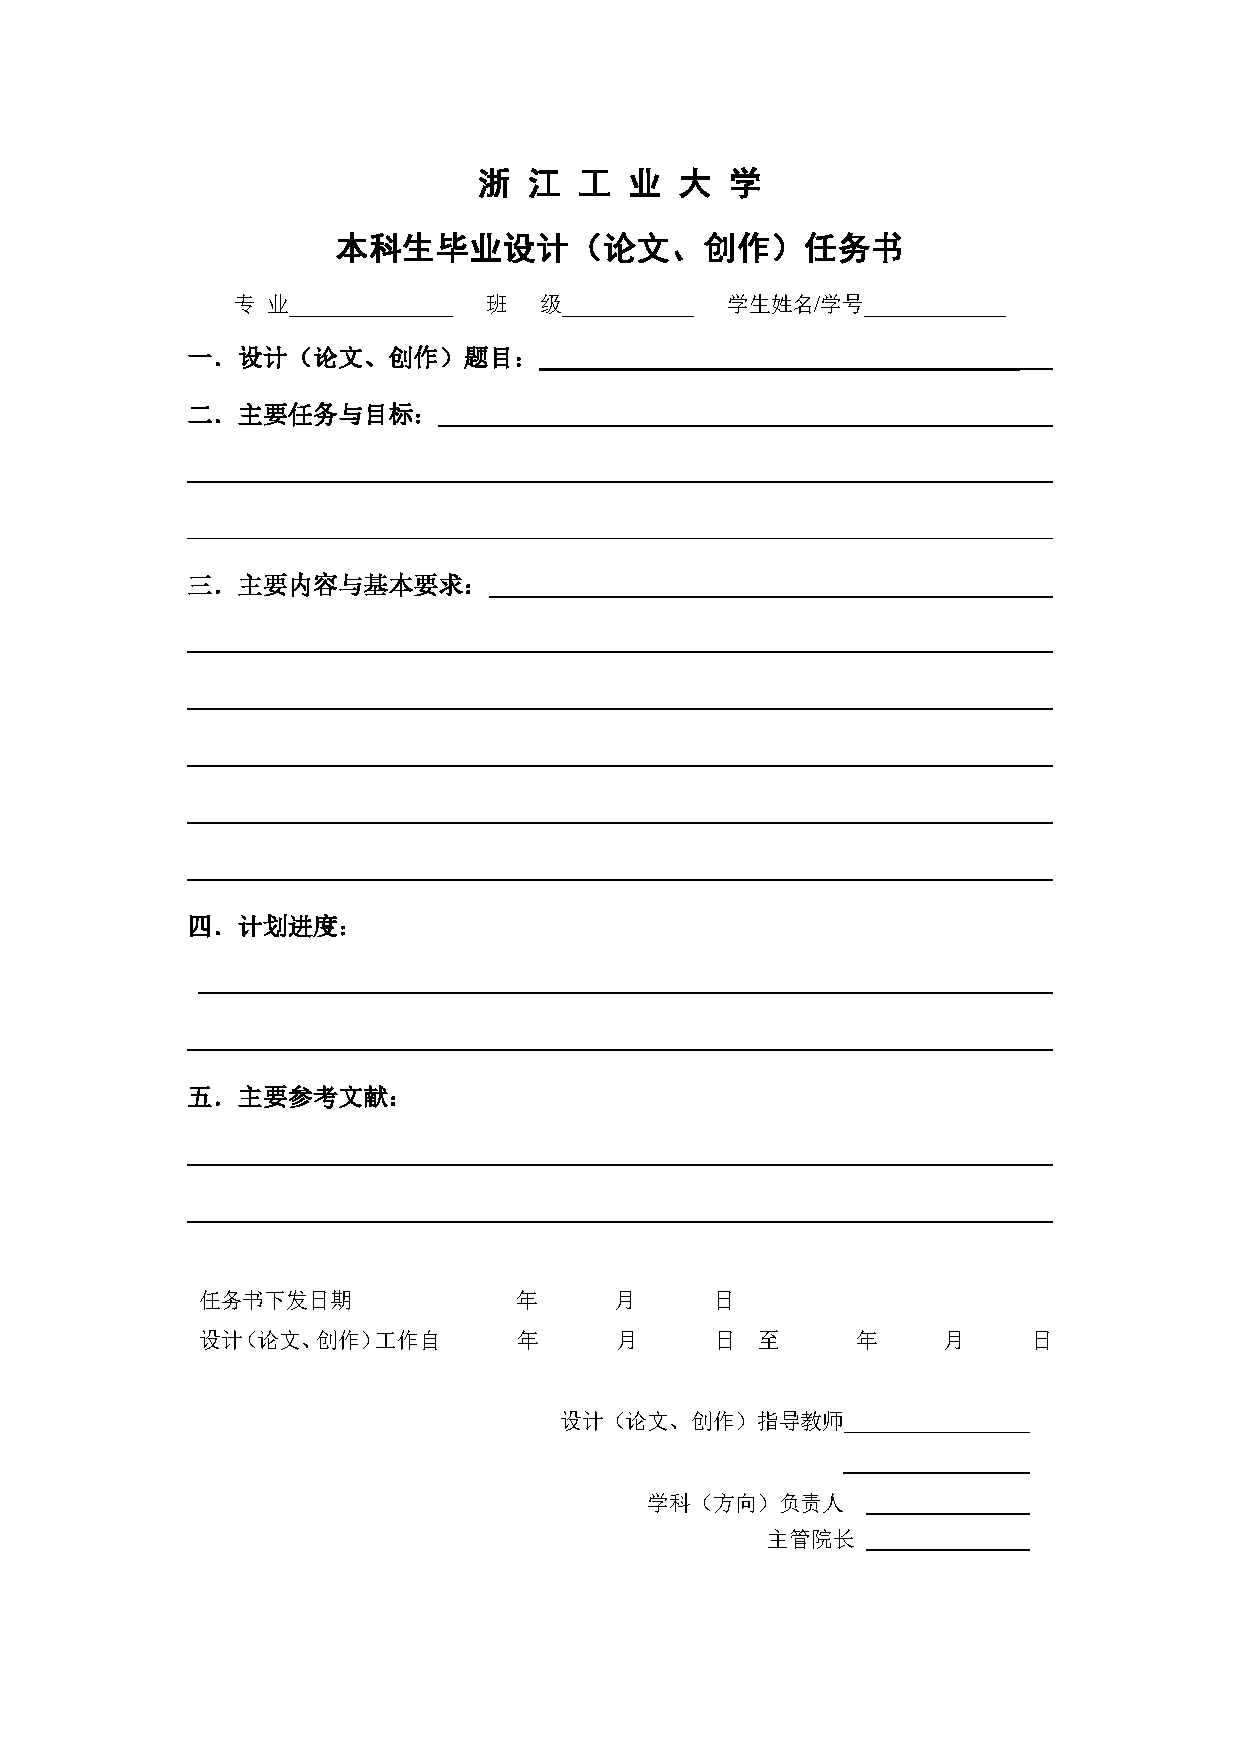
\includepdf{pdf/任务书.pdf}
\end{lstlisting}

\subsection{摘要}

需要在main.tex文件的导言区修改以下个人信息:

\begin{lstlisting}
	%英文摘要信息
	\Enthesis{你的英文摘要标题}
	\Enmyname{你的英文名}
	\Enmysupervisor{导师的英文名}
	\Endepartment{College of Science}
\end{lstlisting}

在\verb|\ZhAbstract{中文摘要内容}{关键词1\hspace{1em}关键词2|中第一个花括号中写入中文摘要,在第二个花括号中填入关键词

在\verb|\EnAbstract{Contents of English Abstract}{Keywords1;Keywords2;}|中第一个花括号中写入英文摘要,在第二个花括号中填入英文关键词


\subsection{目录、图列、表列}

以下是目录、表列、图列的生成,以及之后的页码用阿拉伯数字,不需要更改。不需要人为添加,插入图片、表格时会自动生成索引。

\begin{lstlisting}
	%目录,表列、图列
	\makeTOCandLOTandLOF
	%页码计数器清零,阿拉伯数字
	\setcounter{page}{0}
	\pagenumbering{arabic}
	\newpage
\end{lstlisting}

\subsection{正文}

将源文件分割成若干个文件,例如将每章内容单独写在一个文件中,会大大简化修改和校对的工作。建议把每个章节放在parts文件夹中,用\verb|\input{parts/xxxx}|来导入,不需要加.tex后缀。

\begin{lstlisting}
	\include{parts/第一章}
	\include{parts/第二章}
\end{lstlisting}

\subsection{参考文献}

\verb|\bibliography{bib文件}|更改为你的bib文件,用\verb|\caite{xxx}|在文中引用。浙江工业大学参照《文后参考文献著录规则》(GBT 7714-2005)执行,gbt7714.sty和gbt7714-2005-unsrt.bst文件已在cls文件中定义了格式。以下代码只需改成你的ref.bib文档,不需要后缀

\begin{lstlisting}
	\newpage
	\bibliography{ref}
	\addcontentsline{toc}{section}{参考文献}
\end{lstlisting}

\subsection{致谢}

代码无需修改,修改parts/致谢文件即可。

\begin{lstlisting}
\makeAcknowledge{\input{parts/致谢}}
\end{lstlisting}

\subsection{附录}

有附录的话修改parts/附录,没有附录的话删除本条代码

\begin{lstlisting}
	\makeAppendix{\input{parts/附录}}
\end{lstlisting}

\newpage
\end{lstlisting}

\subsection{参考文献}

\verb|\bibliography{bib文件}|更改为你的bib文件,用\verb|\caite{xxx}|在文中引用。浙江工业大学参照《文后参考文献著录规则》(GBT 7714-2005)执行,gbt7714.sty和gbt7714-2005-unsrt.bst文件已在cls文件中定义了格式。以下代码只需改成你的ref.bib文档,不需要后缀

\begin{lstlisting}
	\newpage
	\bibliography{ref}
	\addcontentsline{toc}{section}{参考文献}
\end{lstlisting}

\subsection{致谢}

代码无需修改,修改parts/致谢文件即可。

\begin{lstlisting}
\makeAcknowledge{谢谢谢谢谢谢谢谢谢谢谢谢谢谢谢谢谢谢谢谢谢谢谢谢谢谢谢谢谢谢谢谢谢谢谢谢谢谢谢谢谢谢谢谢谢谢谢谢谢谢谢谢谢谢谢谢谢谢谢谢谢谢谢谢谢谢谢谢谢谢谢谢谢谢谢谢谢谢谢谢谢谢谢谢谢谢谢谢谢谢谢谢谢谢谢谢谢谢谢谢谢谢谢谢谢谢谢谢谢谢谢谢谢谢谢谢谢谢谢谢谢谢谢谢谢谢谢谢谢谢谢谢谢谢谢谢谢谢谢谢谢谢谢谢谢谢谢谢谢谢谢谢谢谢谢谢谢谢谢谢谢谢谢谢谢谢谢谢谢谢谢谢谢谢谢谢谢谢谢谢谢谢谢谢谢谢谢谢谢谢

谢谢谢谢谢谢谢谢谢谢谢谢谢谢谢谢谢谢谢谢谢谢谢谢谢谢谢谢谢谢谢谢谢谢谢谢谢谢谢谢谢谢谢谢谢谢谢谢谢谢谢谢谢谢谢谢谢谢谢谢谢谢谢谢谢谢谢谢谢谢谢谢谢谢谢谢谢谢谢谢谢谢谢谢谢谢谢谢谢谢谢谢谢谢谢谢谢谢谢谢谢谢谢谢谢谢谢谢谢谢谢谢谢谢谢谢谢谢谢谢谢谢谢谢谢谢谢谢谢谢谢谢谢谢谢谢谢谢谢谢谢谢谢谢谢谢谢谢谢谢谢谢谢谢谢谢谢谢谢谢谢谢谢谢谢谢谢谢谢谢谢谢谢谢谢谢谢谢谢谢谢谢谢谢谢谢谢谢谢谢

谢谢谢谢谢谢谢谢谢谢谢谢谢谢谢谢谢谢谢谢谢谢谢谢谢谢谢谢谢谢谢谢谢谢谢谢谢谢谢谢谢谢谢谢谢谢谢谢谢谢谢谢谢谢谢谢谢谢谢谢谢谢谢谢谢谢谢谢谢谢谢谢谢谢谢谢谢谢谢谢谢谢谢谢谢谢谢谢谢谢谢谢谢谢谢谢谢谢谢谢谢谢谢谢谢谢谢谢谢谢谢谢谢谢谢谢谢谢谢谢谢谢谢谢谢谢谢谢谢谢谢谢谢谢谢谢谢谢谢谢谢谢谢谢谢谢谢谢谢谢谢谢谢谢谢谢谢谢谢谢谢谢谢谢谢谢谢谢谢谢谢谢谢谢谢谢谢谢谢谢谢谢谢谢谢谢谢谢谢谢}
\end{lstlisting}

\subsection{附录}

有附录的话修改parts/附录,没有附录的话删除本条代码

\begin{lstlisting}
	\makeAppendix{\section*{附\hspace{1em}录}		
\addcontentsline{toc}{section}{附录}

附录内容附录内容附录内容附录内容附录内容附录内容附录内容附录内容附录内容附录内容附录内容附录内容附录内容附录内容附录内容附录内容附录内容附录内容附录内容附录内容附录内容附录内容附录内容附录内容附录内容附录内容附录内容附录内容附录内容附录内容附录内容附录内容附录内容附录内容附录内容附录内容附录内容附录内容附录内容附录内容附录内容附录内容附录内容附录内容附录内容附录内容附录内容附录内容附录内容附录内容附录内容附录内容附录内容附录内容附录内容附录内容附录内容附录内容附录内容附录内容附录内容附录内容附录内容附录内容附录内容附录内容附录内容附录内容附录内容附录内容附录内容附录内容附录内容附录内容附录内容附录内容附录内容附录内容附录内容附录内容附录内容附录内容附录内容附录内容附录内容附录内容附录内容附录内容附录内容附录内容附录内容附录内容附录内容附录内容附录内容附录内容附录内容附录内容附录内容附录内容附录内容附录内容附录内容附录内容附录内容附录内容附录内容附录内容}
\end{lstlisting}

\newpage
\end{lstlisting}

\subsection{参考文献}

\verb|\bibliography{bib文件}|更改为你的bib文件,用\verb|\caite{xxx}|在文中引用。浙江工业大学参照《文后参考文献著录规则》(GBT 7714-2005)执行,gbt7714.sty和gbt7714-2005-unsrt.bst文件已在cls文件中定义了格式。以下代码只需改成你的ref.bib文档,不需要后缀

\begin{lstlisting}
	\newpage
	\bibliography{ref}
	\addcontentsline{toc}{section}{参考文献}
\end{lstlisting}

\subsection{致谢}

代码无需修改,修改parts/致谢文件即可。

\begin{lstlisting}
\makeAcknowledge{谢谢谢谢谢谢谢谢谢谢谢谢谢谢谢谢谢谢谢谢谢谢谢谢谢谢谢谢谢谢谢谢谢谢谢谢谢谢谢谢谢谢谢谢谢谢谢谢谢谢谢谢谢谢谢谢谢谢谢谢谢谢谢谢谢谢谢谢谢谢谢谢谢谢谢谢谢谢谢谢谢谢谢谢谢谢谢谢谢谢谢谢谢谢谢谢谢谢谢谢谢谢谢谢谢谢谢谢谢谢谢谢谢谢谢谢谢谢谢谢谢谢谢谢谢谢谢谢谢谢谢谢谢谢谢谢谢谢谢谢谢谢谢谢谢谢谢谢谢谢谢谢谢谢谢谢谢谢谢谢谢谢谢谢谢谢谢谢谢谢谢谢谢谢谢谢谢谢谢谢谢谢谢谢谢谢谢谢谢谢

谢谢谢谢谢谢谢谢谢谢谢谢谢谢谢谢谢谢谢谢谢谢谢谢谢谢谢谢谢谢谢谢谢谢谢谢谢谢谢谢谢谢谢谢谢谢谢谢谢谢谢谢谢谢谢谢谢谢谢谢谢谢谢谢谢谢谢谢谢谢谢谢谢谢谢谢谢谢谢谢谢谢谢谢谢谢谢谢谢谢谢谢谢谢谢谢谢谢谢谢谢谢谢谢谢谢谢谢谢谢谢谢谢谢谢谢谢谢谢谢谢谢谢谢谢谢谢谢谢谢谢谢谢谢谢谢谢谢谢谢谢谢谢谢谢谢谢谢谢谢谢谢谢谢谢谢谢谢谢谢谢谢谢谢谢谢谢谢谢谢谢谢谢谢谢谢谢谢谢谢谢谢谢谢谢谢谢谢谢谢

谢谢谢谢谢谢谢谢谢谢谢谢谢谢谢谢谢谢谢谢谢谢谢谢谢谢谢谢谢谢谢谢谢谢谢谢谢谢谢谢谢谢谢谢谢谢谢谢谢谢谢谢谢谢谢谢谢谢谢谢谢谢谢谢谢谢谢谢谢谢谢谢谢谢谢谢谢谢谢谢谢谢谢谢谢谢谢谢谢谢谢谢谢谢谢谢谢谢谢谢谢谢谢谢谢谢谢谢谢谢谢谢谢谢谢谢谢谢谢谢谢谢谢谢谢谢谢谢谢谢谢谢谢谢谢谢谢谢谢谢谢谢谢谢谢谢谢谢谢谢谢谢谢谢谢谢谢谢谢谢谢谢谢谢谢谢谢谢谢谢谢谢谢谢谢谢谢谢谢谢谢谢谢谢谢谢谢谢谢谢}
\end{lstlisting}

\subsection{附录}

有附录的话修改parts/附录,没有附录的话删除本条代码

\begin{lstlisting}
	\makeAppendix{\section*{附\hspace{1em}录}		
\addcontentsline{toc}{section}{附录}

附录内容附录内容附录内容附录内容附录内容附录内容附录内容附录内容附录内容附录内容附录内容附录内容附录内容附录内容附录内容附录内容附录内容附录内容附录内容附录内容附录内容附录内容附录内容附录内容附录内容附录内容附录内容附录内容附录内容附录内容附录内容附录内容附录内容附录内容附录内容附录内容附录内容附录内容附录内容附录内容附录内容附录内容附录内容附录内容附录内容附录内容附录内容附录内容附录内容附录内容附录内容附录内容附录内容附录内容附录内容附录内容附录内容附录内容附录内容附录内容附录内容附录内容附录内容附录内容附录内容附录内容附录内容附录内容附录内容附录内容附录内容附录内容附录内容附录内容附录内容附录内容附录内容附录内容附录内容附录内容附录内容附录内容附录内容附录内容附录内容附录内容附录内容附录内容附录内容附录内容附录内容附录内容附录内容附录内容附录内容附录内容附录内容附录内容附录内容附录内容附录内容附录内容附录内容附录内容附录内容附录内容附录内容附录内容}
\end{lstlisting}

\newpage
\end{lstlisting}

\subsection{参考文献}

\verb|\bibliography{bib文件}|更改为你的bib文件,用\verb|\cite{xxx}|在文中引用。浙江工业大学参照《文后参考文献著录规则》(GBT 7714-2005)执行,gbt7714.sty和gbt7714-2005-unsrt.bst文件已在cls文件中定义了格式。以下代码只需改成你的ref.bib文档,不需要后缀

\begin{lstlisting}
	\newpage
	\bibliography{ref}
	\addcontentsline{toc}{section}{参考文献}
\end{lstlisting}

\subsection{致谢}

代码无需修改,修改parts/致谢文件即可。

\begin{lstlisting}
\makeAcknowledge{谢谢谢谢谢谢谢谢谢谢谢谢谢谢谢谢谢谢谢谢谢谢谢谢谢谢谢谢谢谢谢谢谢谢谢谢谢谢谢谢谢谢谢谢谢谢谢谢谢谢谢谢谢谢谢谢谢谢谢谢谢谢谢谢谢谢谢谢谢谢谢谢谢谢谢谢谢谢谢谢谢谢谢谢谢谢谢谢谢谢谢谢谢谢谢谢谢谢谢谢谢谢谢谢谢谢谢谢谢谢谢谢谢谢谢谢谢谢谢谢谢谢谢谢谢谢谢谢谢谢谢谢谢谢谢谢谢谢谢谢谢谢谢谢谢谢谢谢谢谢谢谢谢谢谢谢谢谢谢谢谢谢谢谢谢谢谢谢谢谢谢谢谢谢谢谢谢谢谢谢谢谢谢谢谢谢谢谢谢谢

谢谢谢谢谢谢谢谢谢谢谢谢谢谢谢谢谢谢谢谢谢谢谢谢谢谢谢谢谢谢谢谢谢谢谢谢谢谢谢谢谢谢谢谢谢谢谢谢谢谢谢谢谢谢谢谢谢谢谢谢谢谢谢谢谢谢谢谢谢谢谢谢谢谢谢谢谢谢谢谢谢谢谢谢谢谢谢谢谢谢谢谢谢谢谢谢谢谢谢谢谢谢谢谢谢谢谢谢谢谢谢谢谢谢谢谢谢谢谢谢谢谢谢谢谢谢谢谢谢谢谢谢谢谢谢谢谢谢谢谢谢谢谢谢谢谢谢谢谢谢谢谢谢谢谢谢谢谢谢谢谢谢谢谢谢谢谢谢谢谢谢谢谢谢谢谢谢谢谢谢谢谢谢谢谢谢谢谢谢谢

谢谢谢谢谢谢谢谢谢谢谢谢谢谢谢谢谢谢谢谢谢谢谢谢谢谢谢谢谢谢谢谢谢谢谢谢谢谢谢谢谢谢谢谢谢谢谢谢谢谢谢谢谢谢谢谢谢谢谢谢谢谢谢谢谢谢谢谢谢谢谢谢谢谢谢谢谢谢谢谢谢谢谢谢谢谢谢谢谢谢谢谢谢谢谢谢谢谢谢谢谢谢谢谢谢谢谢谢谢谢谢谢谢谢谢谢谢谢谢谢谢谢谢谢谢谢谢谢谢谢谢谢谢谢谢谢谢谢谢谢谢谢谢谢谢谢谢谢谢谢谢谢谢谢谢谢谢谢谢谢谢谢谢谢谢谢谢谢谢谢谢谢谢谢谢谢谢谢谢谢谢谢谢谢谢谢谢谢谢谢}
\end{lstlisting}

\subsection{附录}

有附录的话修改parts/附录,没有附录的话删除本条代码

\begin{lstlisting}
	\makeAppendix{\section*{附\hspace{1em}录}		
\addcontentsline{toc}{section}{附录}

附录内容附录内容附录内容附录内容附录内容附录内容附录内容附录内容附录内容附录内容附录内容附录内容附录内容附录内容附录内容附录内容附录内容附录内容附录内容附录内容附录内容附录内容附录内容附录内容附录内容附录内容附录内容附录内容附录内容附录内容附录内容附录内容附录内容附录内容附录内容附录内容附录内容附录内容附录内容附录内容附录内容附录内容附录内容附录内容附录内容附录内容附录内容附录内容附录内容附录内容附录内容附录内容附录内容附录内容附录内容附录内容附录内容附录内容附录内容附录内容附录内容附录内容附录内容附录内容附录内容附录内容附录内容附录内容附录内容附录内容附录内容附录内容附录内容附录内容附录内容附录内容附录内容附录内容附录内容附录内容附录内容附录内容附录内容附录内容附录内容附录内容附录内容附录内容附录内容附录内容附录内容附录内容附录内容附录内容附录内容附录内容附录内容附录内容附录内容附录内容附录内容附录内容附录内容附录内容附录内容附录内容附录内容附录内容}
\end{lstlisting}

\newpage